\documentclass[runningheads]{llncs}
\usepackage[T1]{fontenc}
\usepackage{graphicx}
%\usepackage{amssymb,amsmath,amsthm,mathtools}
\usepackage{amssymb,amsmath}

\newtheorem{cor}[theorem]{Corollary}

%\documentclass{article}
%\usepackage{graphicx} 
%\usepackage{fullpage}
%\usepackage{amssymb,amsmath,amsthm,mathtools}

\usepackage{hyperref}

%\newtheorem{theorem}{Theorem}
%\newtheorem{thm}[theorem]{Theorem}
%\newtheorem{lemma}[theorem]{Lemma}
%\newtheorem{cor}[theorem]{Corollary}
%\newtheorem{obs}[theorem]{Observation}
%\newtheorem{conj}[theorem]{Conjecture}
%\newtheorem{dfn}[theorem]{Definition}
%\newtheorem{prob}[theorem]{Problem}
\newtheorem{prop}[theorem]{Proposition}
%\newtheorem{claim}[theorem]{Claim}

\newcommand{\etal}{\emph{et al.}}

\begin{document}

\title{Generalized Kendall $\tau$}
\author{Sergey Bereg\inst{1}%\orcidID{0000-1111-2222-3333} 
\and
Nhat Vu Minh Truong\inst{1}%\orcidID{1111-2222-3333-4444} 
}

\date{June 2025}


\institute{Department of Computer Science,
University of Texas at Dallas,
Box 830688,
Richardson, TX 75083
USA.
}

\maketitle

% -----------------------------
\section{Introduction}
Generalized Kendall Tau for partial rankings [1]

Wang \etal \cite{wang24} consider a generalized Kendall‑$\tau$ metric and permutation codes using it as well as Levenshtein and Ulam metrics.

The {\em generalized Kendall $\tau$ distance} between two permutations $\pi, \sigma \in S_n$, denoted by $d_T(\pi, \sigma)$, is defined as the minimum number of translocations required to transform $\pi$ into $\sigma$.
We call it the {\em T-distance} for short.

For an array $A$ of permutations, the pairwise T-distance of $A$, denoted by $d(A)$, 
is $\min \{ ~d_T(\sigma,\pi)~ |~ \sigma, \pi \in A, \sigma\ne \pi ~ \}$. 
An {\em $(n,d)$-PA} is an array $A$ of permutations on $[1...n]$ with $d_T(A)\ge d$. 
Let $T(n,d)$ be the maximum size of a $(n,d)$-PA under the generalized Kendall $\tau$ metric.


NP-hard \cite{bult12}

% -----------------------------
\section{Graphs $G_n$ and $G_{n,d}$}

We define a graph $G_n$ where the vertices are the permutations of $[1..n]$ and two permutations $\pi$ and $\sigma$ are connected by an edge if $\sigma$ can be obtained from $\pi$ by a translocation.
We also define a graph $G_{n,d}$ where the vertices are the permutations of $[1..n]$ and two permutations $\pi$ and $\sigma$ are connected by an edge if $d_T(\pi,\sigma)\ge d$.

\begin{prop}
\label{prop1}
(i) For all $n\ge 3$, $G_n$ is a regular graph of degree $\binom{n+1}{3}$.
%There $\binom{n+1}{3}$ ways for the first translocation in $\pi\to \sigma$.
\\
(ii) For all $n\ge 3$ and $2\le d\le 2n-2$,
graph $G_{n,d}$ is the complement of $(G_{n,1})^{d-1}$, i.e. 
$G_{n,d}=\overline{(G_n)^{d-1}}$.
\end{prop}

%A graph $G_{n,d}$ for $d\ge 2$ can be viewed as $G_{n,d}=(G_{n,1})^d$.

\begin{proof}
..    
\end{proof}

We will use graphs $G_n$ and $G_{n,d}$ to obtain exact values of $T(n,d)$ or bounds on $T(n,d)$.
Observe that $T(n,1)=n!$ for all $n\ge 1$ since at least one translocation is required to transform a permutation $\pi\in S_n$ to another permutation $\sigma\in S_n$. 

\begin{theorem}
$T(4,2)=4$ and $T(4,3)=2$.    
\end{theorem}

\begin{proof}
Consider graph $G_4$. 
By Proposition \ref{prop1}, $G_4$ is a regular graph of degree $\binom{5}{3}=10$ with $4!=24$ vertices.
The neighborhood of permutation $(1,2,3,4)$ or 1234 for short is $N(1234)=\{2134, 1324, 1243, 2314, 3124, 1342, 1423, 2143, 2341, 4123\}$ and the neighborhood of 4321 is $N(4321)=\{...\}$. 
Since these neigborhoods are disjoint and each vertex has degree 10, $G_{4}-\{1234,4321\}$ is ...
, see Fig. \ref{f1}.

First, we show $T(4,3)=2$.
Consider a $(4,3)$-array $P$.
Without loss of generality, the identity permutation is in $P$, i.e. $1234\in P$. 
The only vertex in $G_4$ at distance 3 from the identity permutation is $4321$. 
Therefore $T(4,3)=2$ for $P=\{1234,4321\}$.

Next, we prove $T(4,2)=4$.
It can be verified that $\{1234,4321,2413,3142\}$ is a $(4,2)$-array. Therefore $T(4,2)\ge 4$.  

To show $T(4,2)\le 4$, consider a $(4,3)$-array $P$.
Again, we can assume that $1234\in P$.
If $4321\in P$ then 
\[ S_4\setminus (\{1234,4321\}\cup N(1234)\cup N(4321)) = \{2413,3142\}\]
and $|P|\le 4$.
Now, we assume that $4321\notin P$.
Suppose $2413\in P$. 
By symmetry we can assume that $3142\notin P$.
Then $P\setminus\{1234,2413\}\subseteq D$, see Fig. \ref{f1}.
Since the subgraph of $G_4$ induced by $D$ is a 5-cycle, at most 2 vertices of $D$ can be in $P$.
Therefore $|P|\le 4$.

It remains to consider the case where $1234\in A$ and 
$\{4321,2413,3242\}\notin A$.
Then $A\setminus\{1234\}\subseteq C\cup D$, see Fig. \ref{f1}. 
The subgraph of $G_4$ induced by $C$ (resp. by $D$) is 5-cycle. 
Then $|P\cap C|\le 2$ and $|P\cap D|\le 2$.
Thus $|P|\le 5$.

Suppose to the contrary that $|P|=5$.
Then $|P\cap C|=2$ and $|P\cap D|=2$.
The graph $G_{C\cup D}$ induced by $C\cup D$ is shown in Fig. \ref{f55} where the 5 cycles of $C$ and $D$ are shown in red and blue.
The graph $G_{C\cup D}$ contains 3-cycle ..., 3-c-cycle ... and 4-cycle ...
$P\cap (C\cup D)$ is an independent set in graph $G_{C\cup D}$.
If an independent set $I$ in $G_{C\cup D}$ has  4 vertices, then $I$ has exactly one vertex from each 3-cycle and 2 vertices from the 4-cycle. There are 2 cases.

Case 1. $2314,3421\in I$. 
Then no vertex in $C$ (the blue cycle) can be in $I$. This contradicts $|P\cap C|=2$.

Case 2. $3214,4231\in I$. 
Then $I$ doesn't contain a vertex in $\{1423,2314,3124\}$. $I$ contains only one of the remaining vertices in $C$. This contradicts $|P\cap C|=2$.
\qed\end{proof}

\begin{figure}[ht]
  \centering
  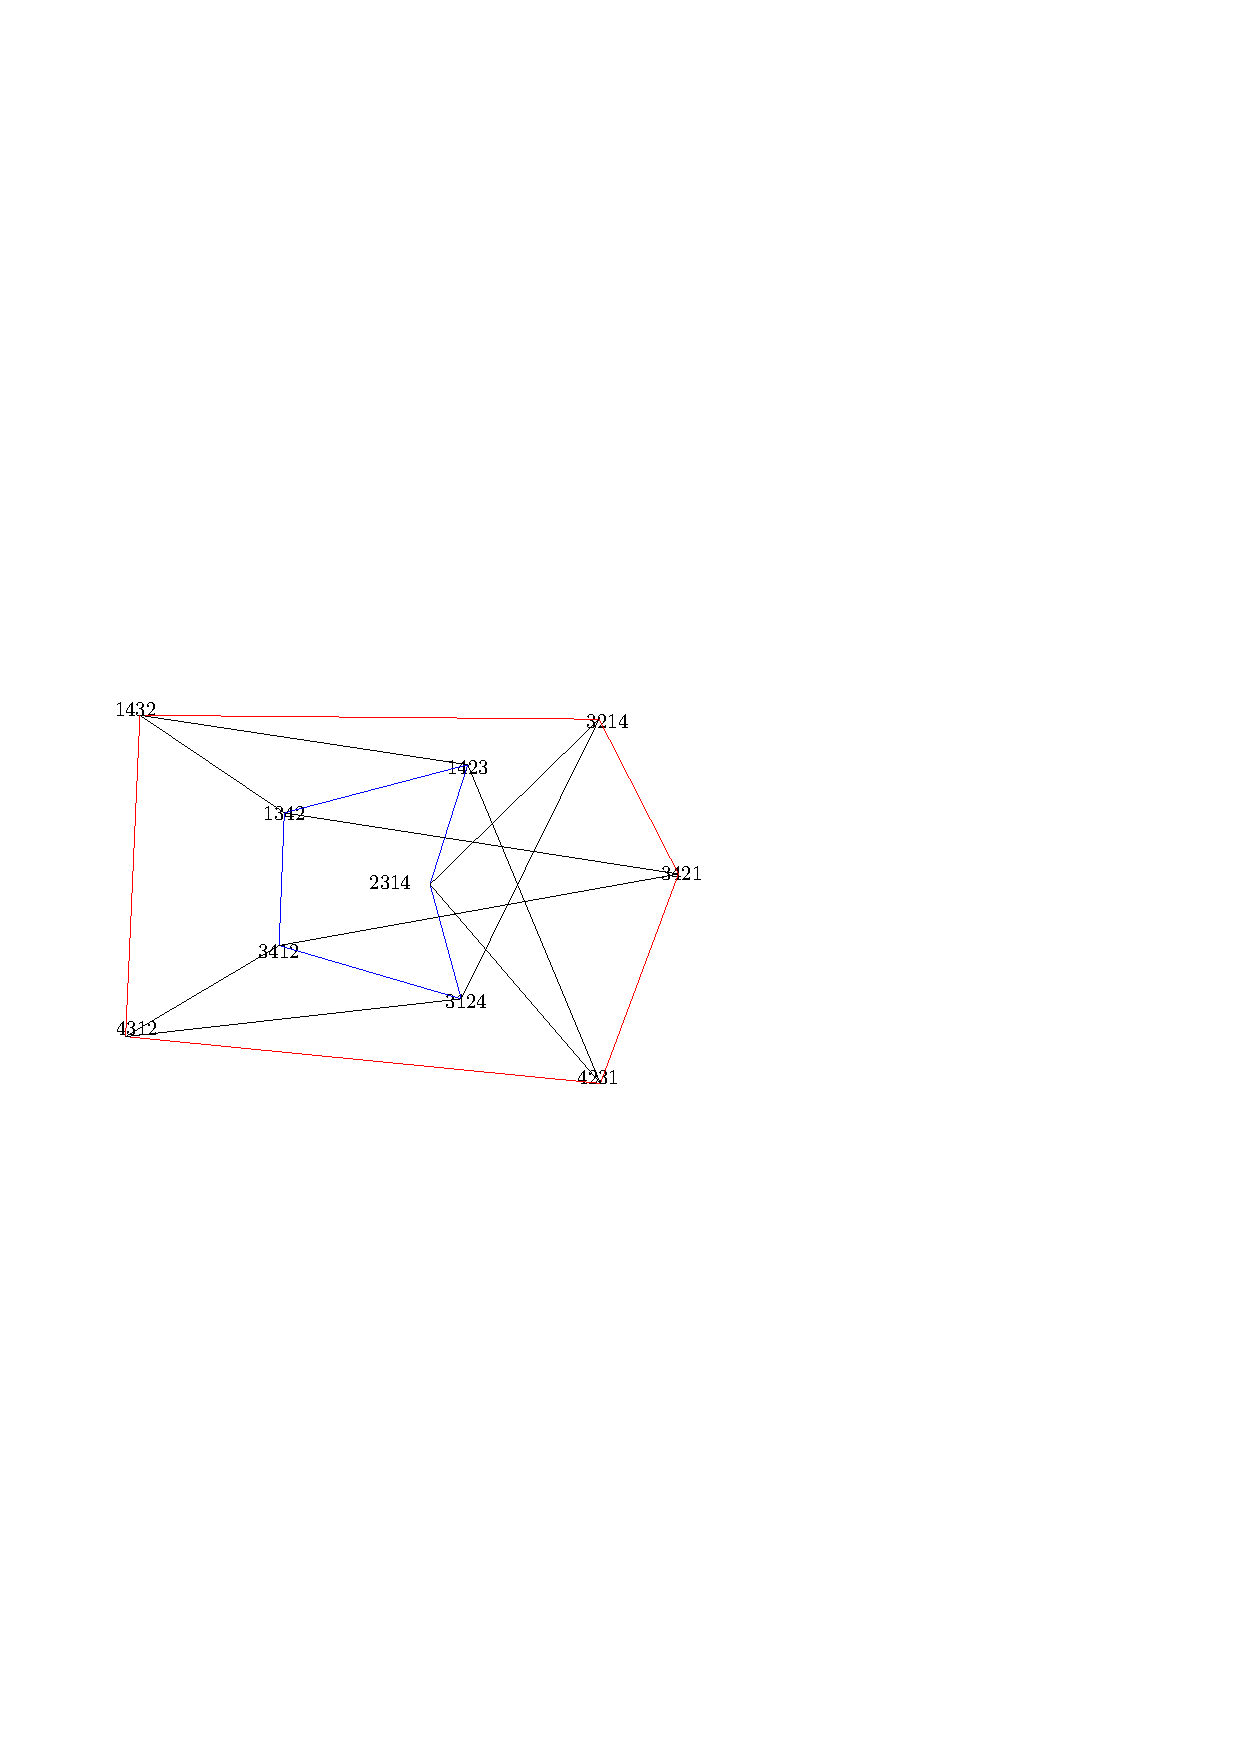
\includegraphics[scale=0.7]{f55.pdf}
  \caption{The graph $G_{C\cup D}$.}
  \label{f55}
\end{figure}


\begin{figure}[ht]
  \centering
  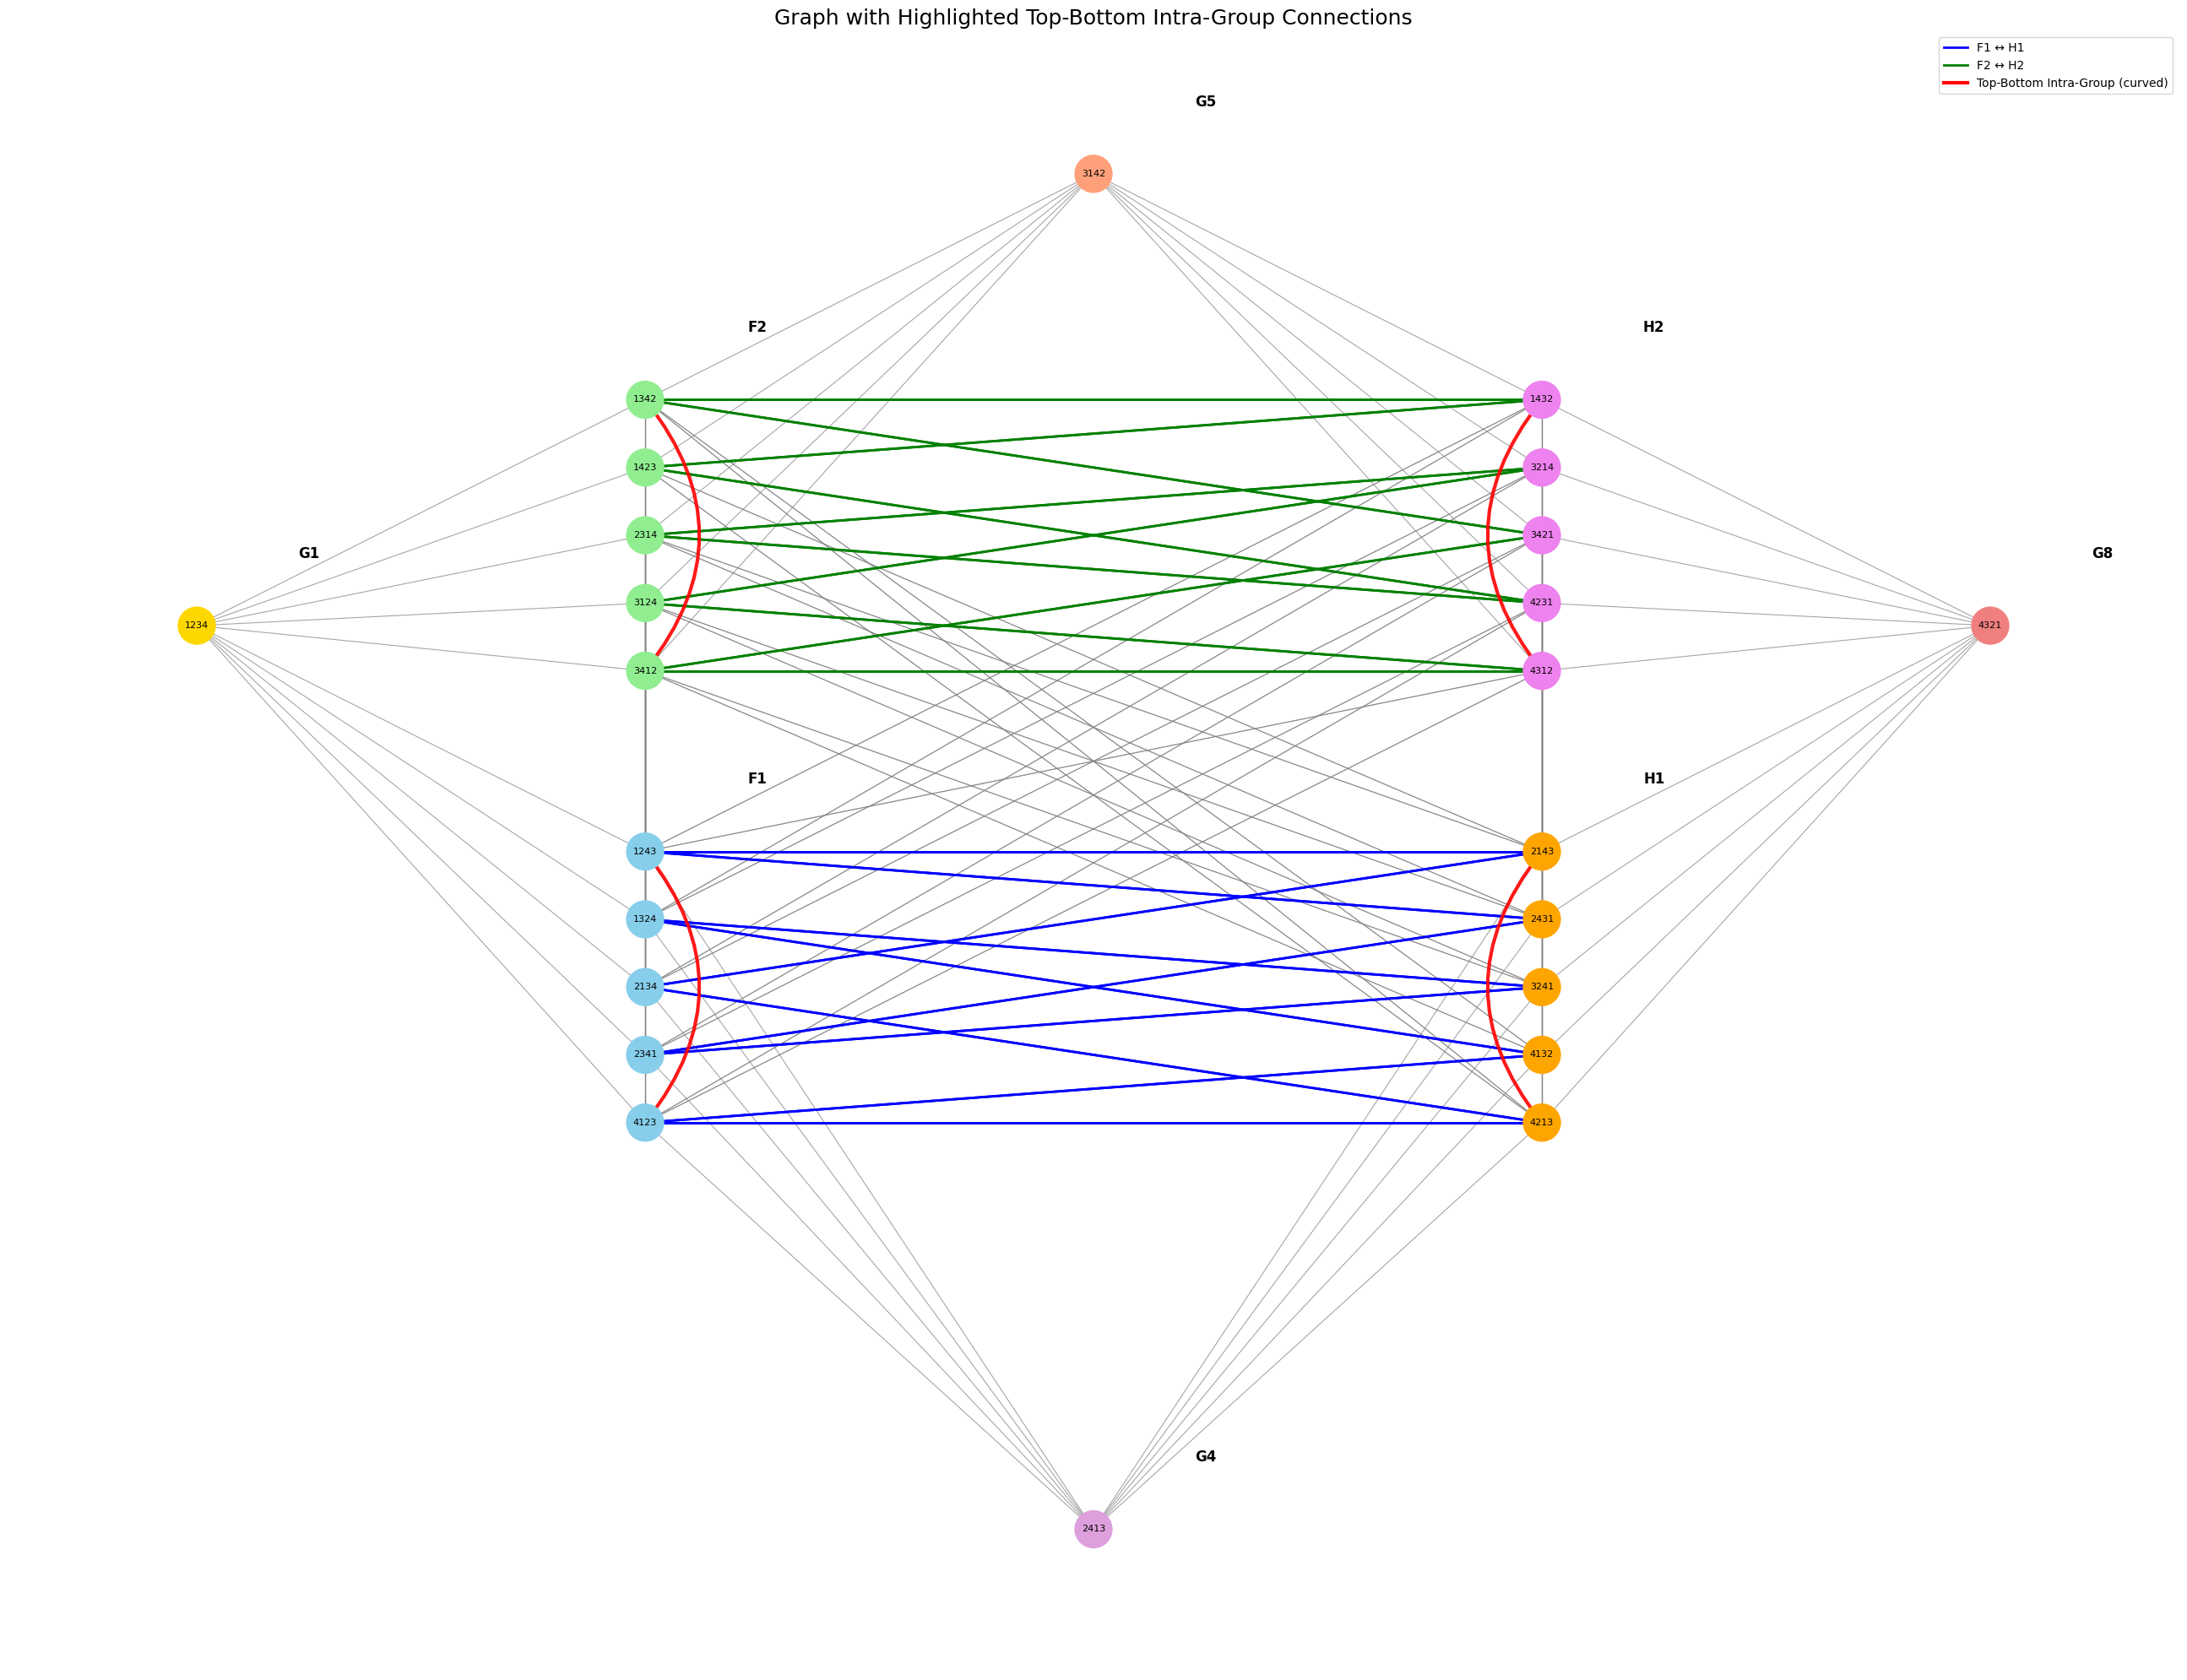
\includegraphics[scale=0.1]{G4.png}
  \caption{The graph $G_{4}$}
  \label{G4}
\end{figure}

\begin{figure}[ht]
  \centering
  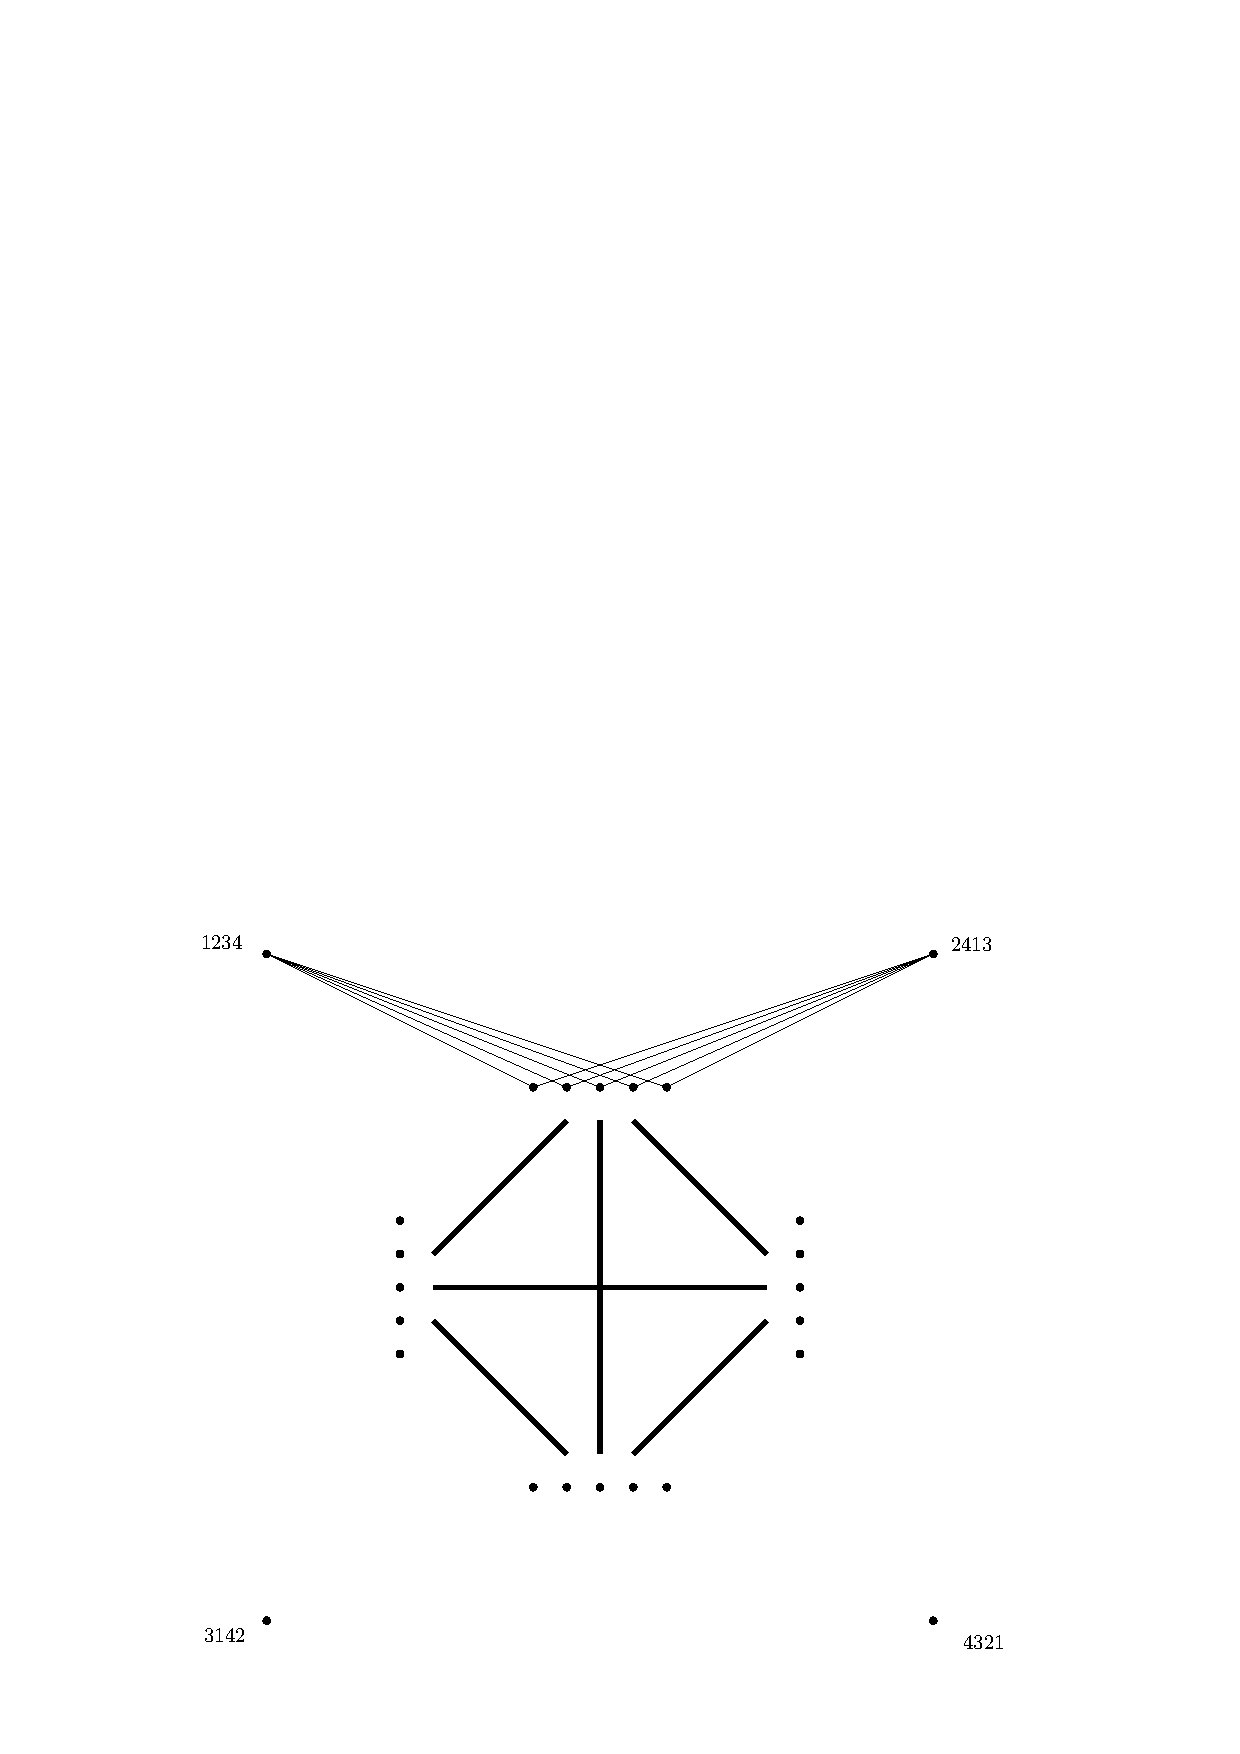
\includegraphics[scale=0.7]{G4.pdf}
  \caption{The graph $G_{4}$}
  \label{G4}
\end{figure}

\begin{figure}[ht]
  \centering
  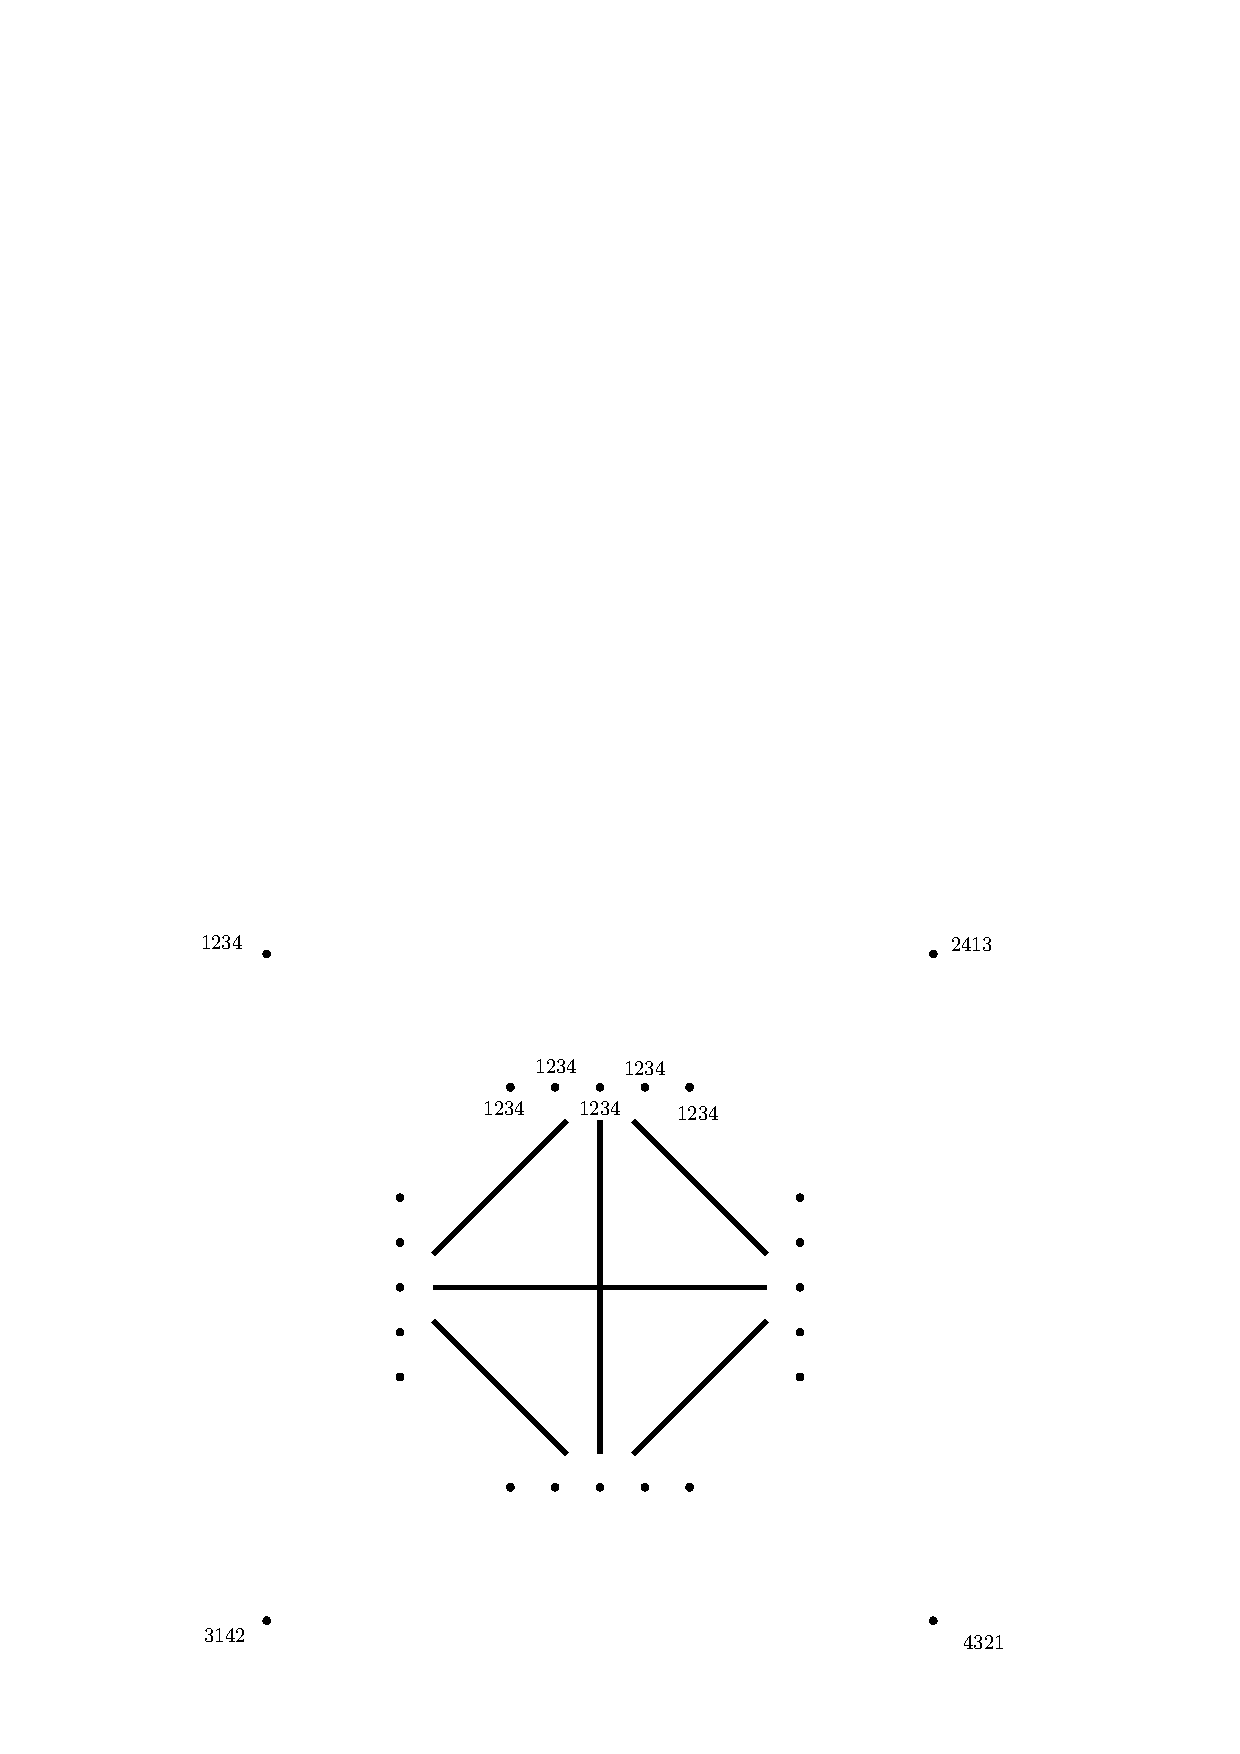
\includegraphics[scale=0.4]{G4a.pdf}
  \caption{The graph $G_{4}$}
  \label{G4}
\end{figure}


\begin{figure}[ht]
  \centering
  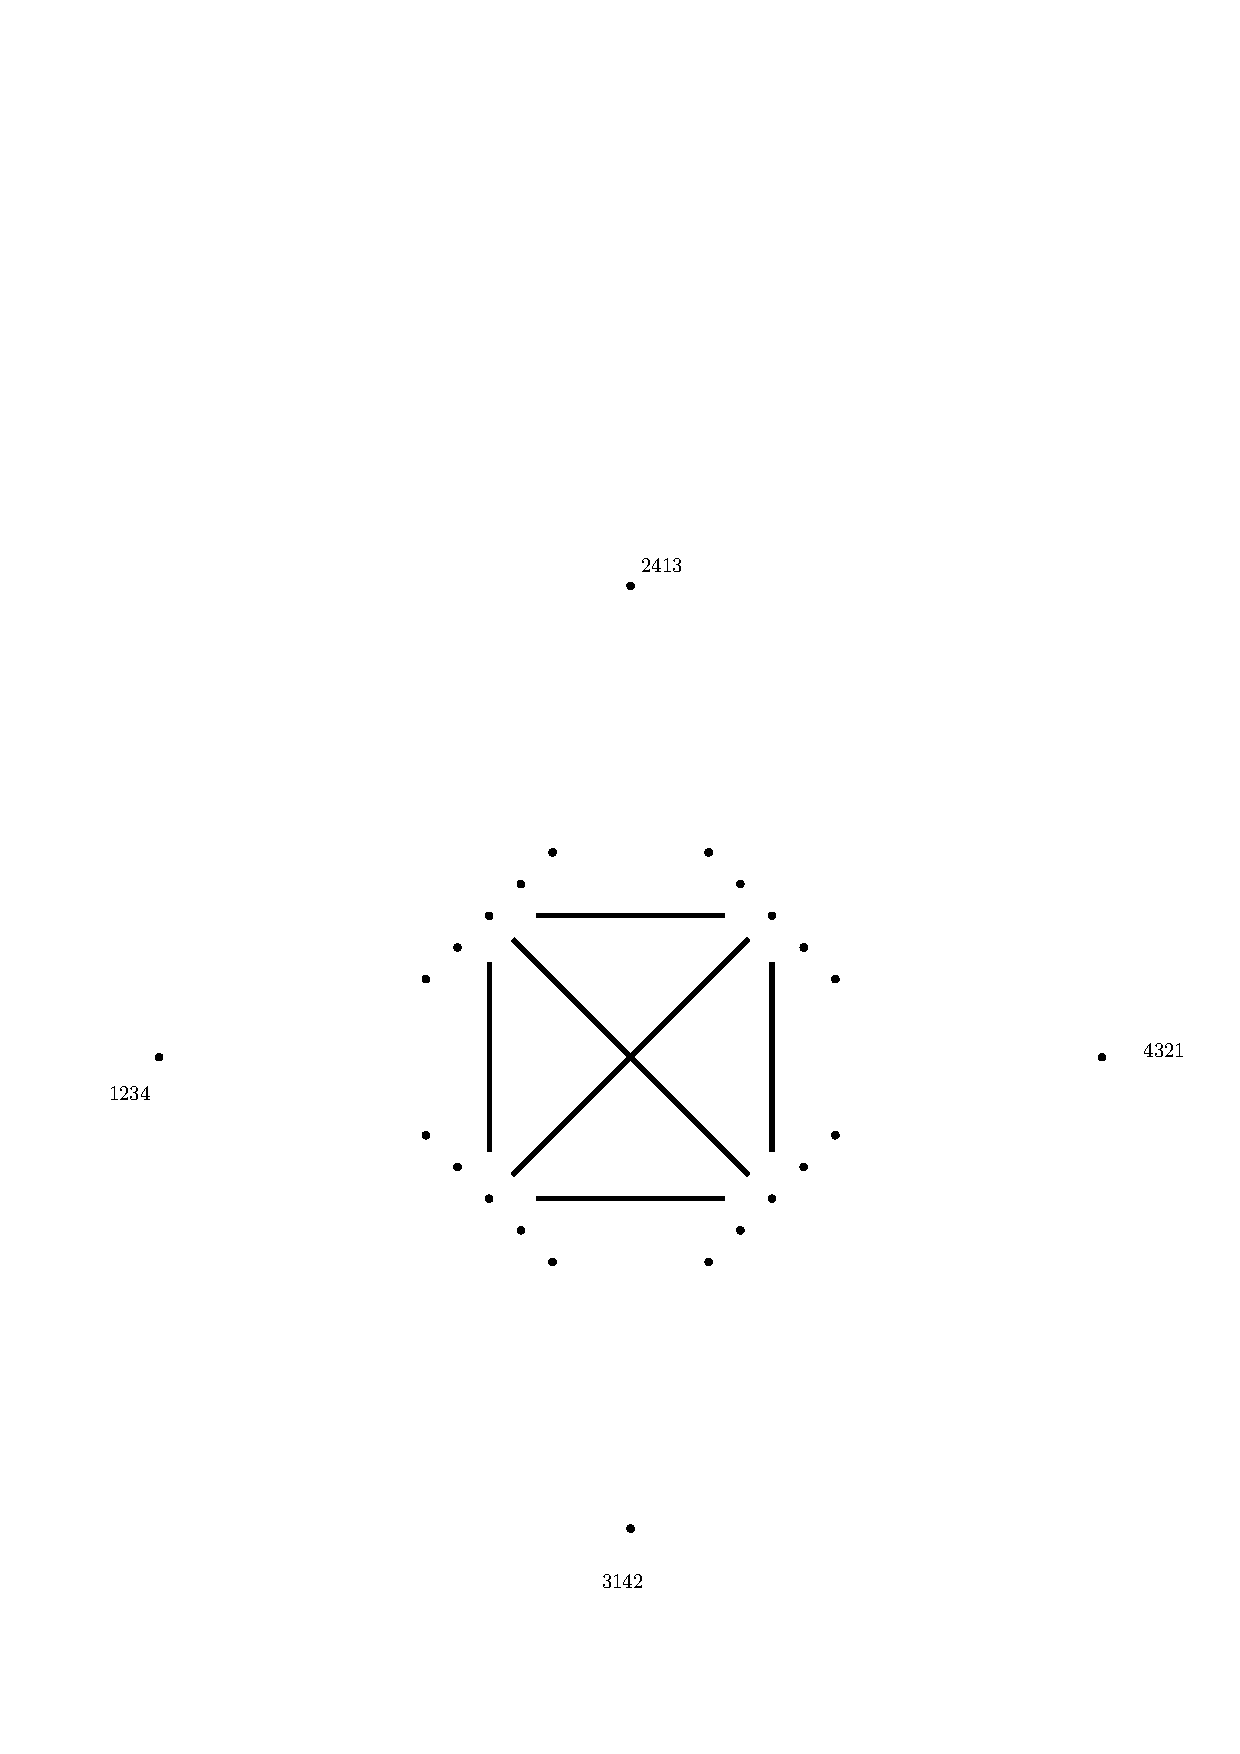
\includegraphics[scale=0.5]{G4b.pdf}
  \caption{The graph $G_{4}$}
  \label{G4}
\end{figure}



\begin{figure}[ht]
  \centering
  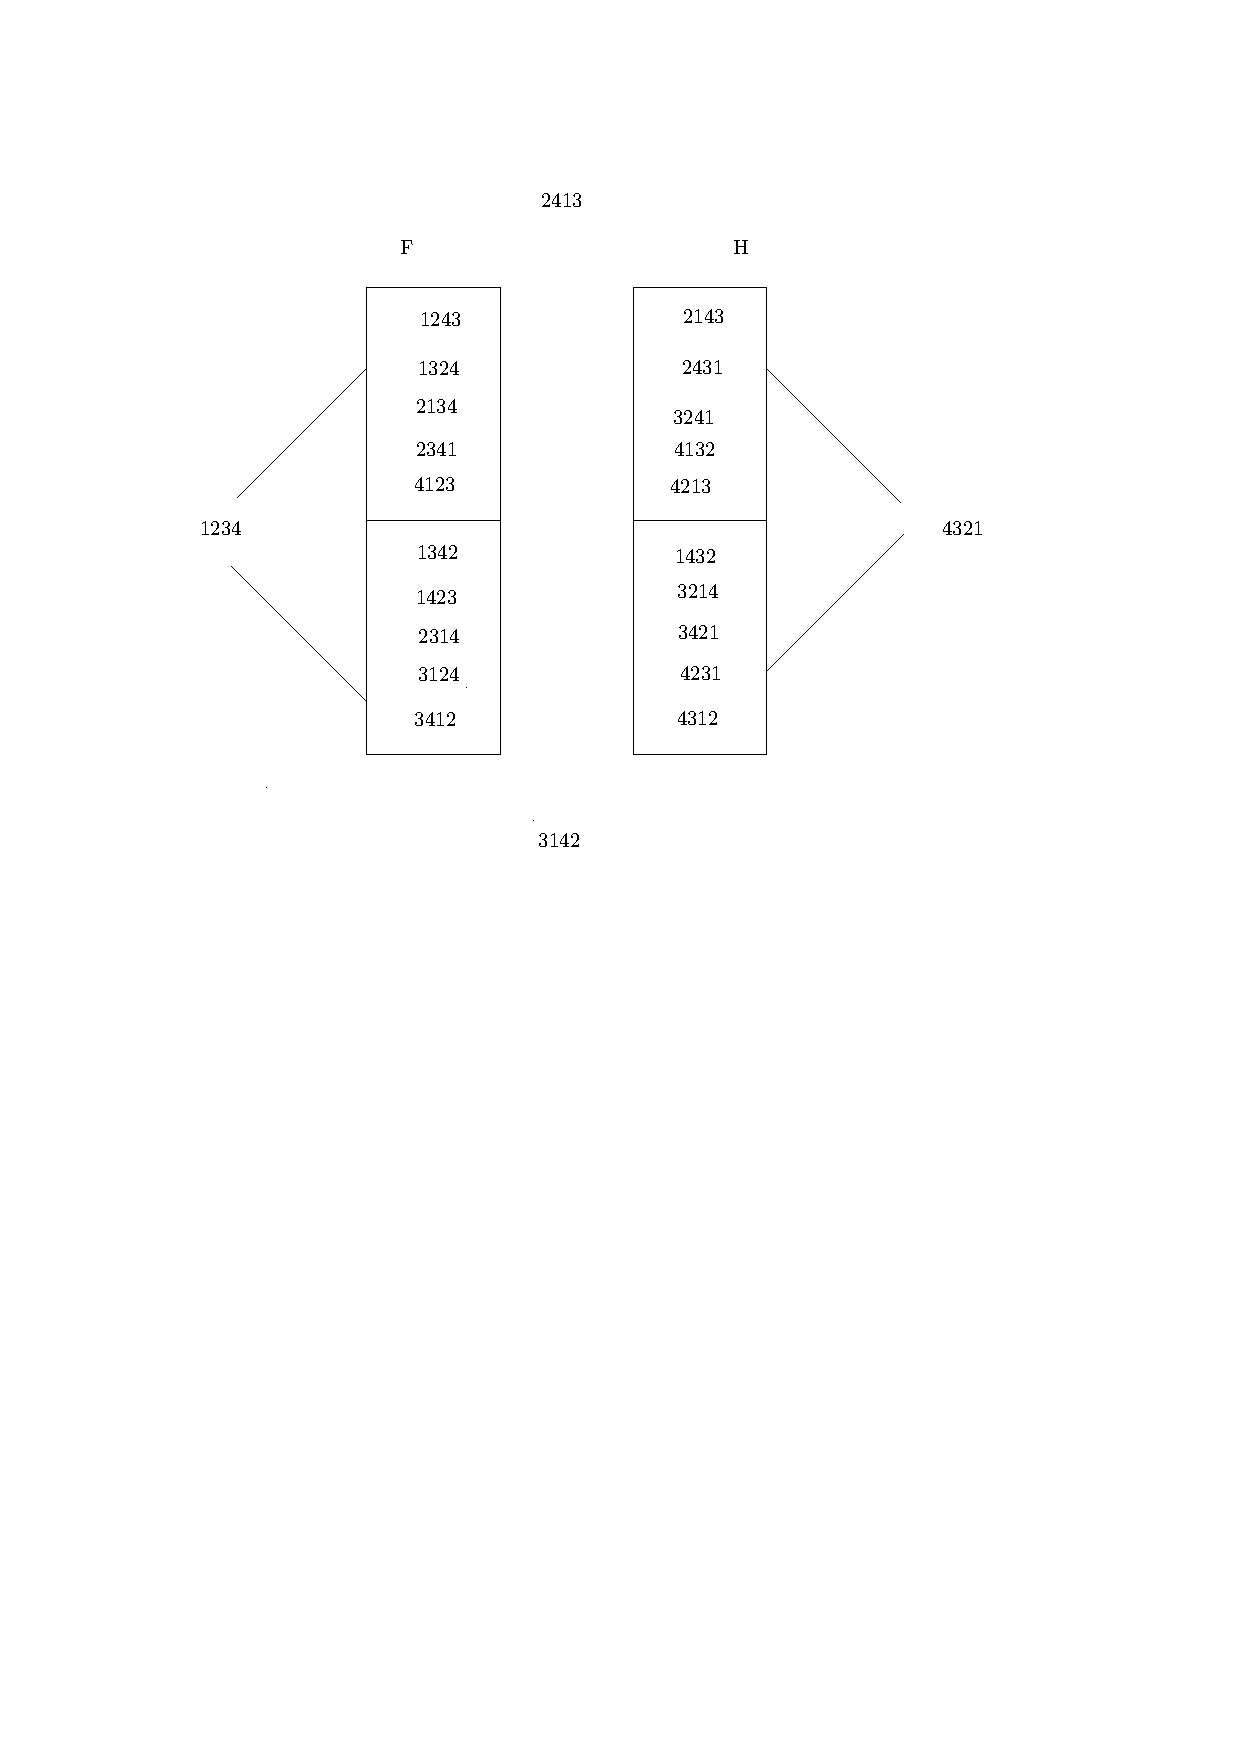
\includegraphics{f1_v2.pdf}
  \caption{The graph $G_{4}$ where $G_{4}-\{1234,4321\}$ has two sugraphs $F$ and $H$.
  2413 - 3412}
  \label{f1}
\end{figure}



\begin{figure}[ht]
  \centering
  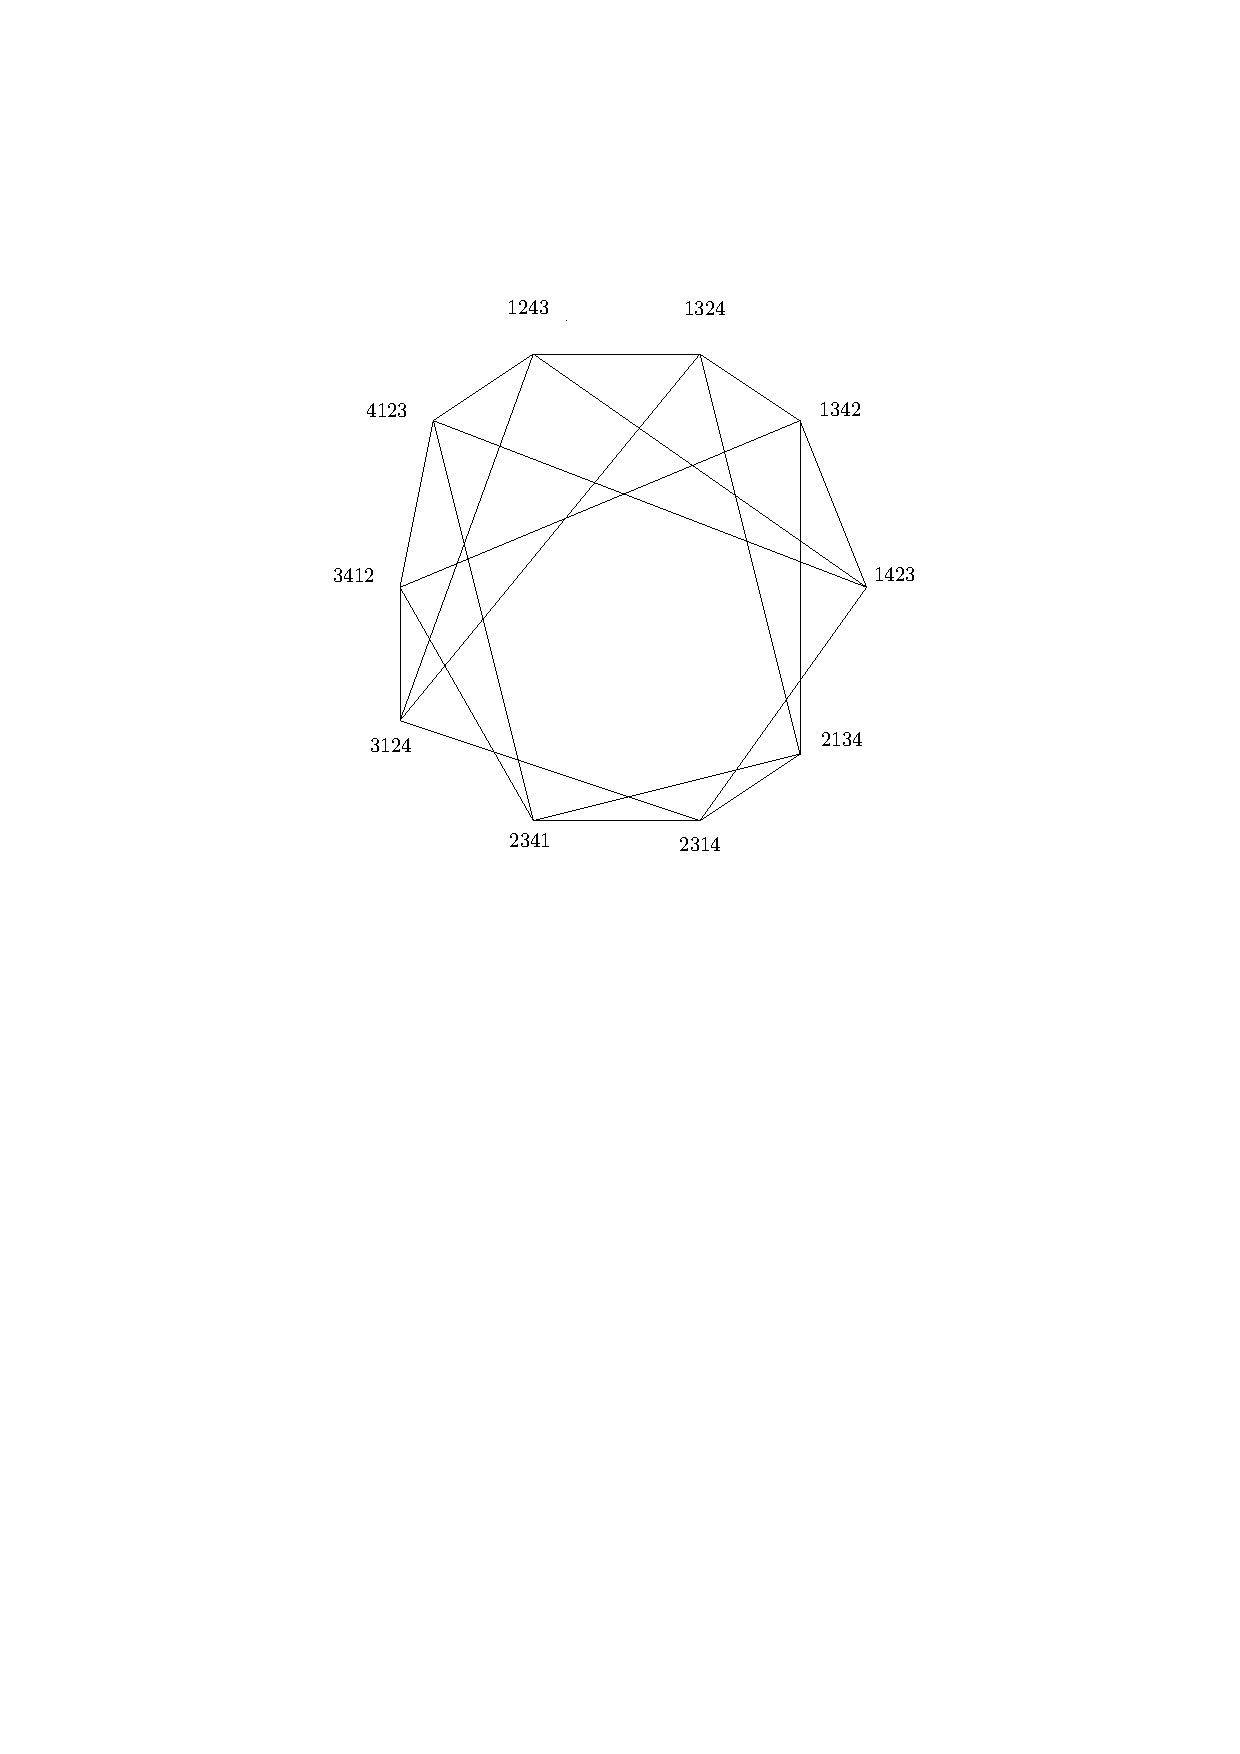
\includegraphics{f2-modified.pdf}
  \caption{The graph $F$, the subgraph of $G_{4}$.}
  \label{f2}
\end{figure}

\section*{Methods}

The sorting problem (given a permutation $\pi$, find min number of gen.adjacent translocations to transform $\pi$ to 1,2,..,n) is NP-hard. 
It is interesting to find permutations with max distance to 1,2,..,n.
Or in general, find distances to 1,2,..,n for all permutations of [1,n]. 

Algorithm:

Make a list of all permutations of $\{1,2,..,n\}$ and set distance $D[\pi]$ as 0 for $\pi=(1,2,..,n)$ and a large int $X$ for other permutations $\pi$.

for dist=0 by 1 to infty\\
for each permutation $\pi$\\
if $D[\pi]=dist$ try every possible adjacent translocation on $\pi$ making a new permutation $\sigma$.\\
If $D[\sigma]=X$ set $D[\sigma]=dist+1$.\\
If $\pi$ is not found for dist then stop

\section*{Glossary}
\textbf{Translocation:} swapping two consecutive sequences. \\
\textbf{Translocation distance:} is the minimum number of operation that are needed to transform one permutation into another. \\
\textbf{Partial Ranking:} 

\vspace{0.5cm}

% ---------------------------------
\section{Computational Result}

\section{Results}

\begin{proof}
The first translocation is defined by $1\le i<j\le k\le n$ using intervals $[i,j-1]$ and $[j,k]$. 
There $\binom{n+1}{3}$ ways for this.
\end{proof}

\begin{theorem}
$d(\pi,\sigma)=n-1$ for $\pi=(1,2,\dots,n)$ and $\sigma=(n,n-1,\dots,1)$.
\end{theorem}

\begin{proof}
{\em Upper bound}. 
We prove by induction that $d(\pi,\sigma)\le n-1$. 

\textbf{Base case}. If $n=1$ then $\pi$ = (1) = $\sigma$ and no translocation needed.

\textbf{Inductive step}.
Suppose $d(\pi,\sigma)\le n-1$.
Let $\pi'=(1,2,\dots,n-1)$ and $\sigma'=(n-1,n-2,\dots,1)$.
We prove $d(\pi,\sigma)\le n-1$ assuming that $d(\pi',\sigma')\le n-2$.

We make a translocation of $n$ and $(1,2,...,n-1)$ in $\pi$ producing permutation $(n, 1, 2, \dots, n-1)$.
It is $\pi'$ after $n$ and we can apply $n-2$ translocations to transform it to $\sigma'$ by induction hypothesis. 
This results in $n-1$ translocations transforming $\pi$ to $\sigma$.

{\em Lower bound}. ...
\end{proof}

\textbf{Proof of lower bound: }{\bf $d(\pi,\sigma) \geq n-1$} \\

\textbf{Base case:} n = 1 \\

$\pi$ = (1) = $\sigma$, no translocation needed.

n - 1 = 0

$d(\pi,\sigma) = 0 \geq 0$\\

\textbf{Assume} n = k 

d((1,2,..k), (k, k-1,...,1)) $\geq$ k-1\\

\textbf{Inductive step:} n = k + 1 

\textbf{Prove} d((1,2,...,k+1), (k+1, k, ..., 1)) $\geq$ k:

To reverse (1,2,...,k+1) to (k+1, k, ..., 1), we make translocation k+1 and (1,2,...,k). 

(1,2,..., k, k+1) now become (k+1, 1, 2, ... k) 

We are left with reversing (1,2,...,k) to (k, ..., 2, 1)

d((1,2,..k+1), (k+1, ..., 2, 1)) = 1+ d(1,2, ..., k),(k, ..., 2, 1) = 1 + k -1 = k = k + 1 - 1 = n - 1 $\geq$ n - 1

\textbf{We proved} {\bf $d(\pi,\sigma) \geq n-1$} 

\vspace{0.5cm}
\textbf{Proof of upper bound: }{\bf $d(\pi,\sigma) \leq n-1$} \\

\textbf{Base case:} n = 1 \\

$\pi$ = (1) = $\sigma$, no translocation needed.

n - 1 = 0

$d(\pi,\sigma) = 0 \leq 0$\\

\textbf{Assume} n = k 

d((1,2,..k), (k, k-1,...,1)) $\leq$ k-1\\

\textbf{Inductive step:} n = k + 1 

\textbf{Prove} d((1,2,...,k+1), (k+1, k, ..., 1)) $\leq$ k:

To reverse (1,2,...,k+1) to (k+1, k, ..., 1), we make translocation k+1 and (1,2,...,k). 

(1,2,..., k, k+1) now become (k+1, 1, 2, ... k) 

We are left with reversing (1,2,...,k) to (k, ..., 2, 1)

d((1,2,..k+1), (k+1, ..., 2, 1)) = 1+ d(1,2, ..., k),(k, ..., 2, 1) = 1 + k -1 = k = k + 1 - 1 = n - 1 $\leq$ n - 1

\textbf{We proved} {\bf $d(\pi,\sigma) \leq n-1$} \\

Therefore, we proved \textbf{Claim 1}  $d(\pi,\sigma)=n-1$ for $\pi=1,2,...$ and $\sigma=...2,1$.\\



When n = 4, we have 16 distinct ways of using exact 3 adjacent interval translocation:

Either moving 4 first and last in the translocation
4123 $->$ 4312 $->$ 4321

4123 $->$ 4213 $->$ 4321

4123 $->$ 4132 $->$ 4321

4123 $->$ 4231 $->$ 4321

3124 $->$ 3214 $->$ 4321

2134 $->$ 3214 $->$ 4321

1324 $->$ 3214 $->$ 4321

2314 $->$ 3214 $->$ 4321

Move 4 in others steps in the translocation 

Move 3 in the front:

(This seems not to work)

\rule{8cm}{0.4pt}

1234

- First move have 4 in the front:
Has 4 remain untouch, there is not possible way to include 4 in other translocation

1. 4123 $->$ 4312 $->$ 4321

2. 4123 $->$ 4213 $->$ 4321

3. 4123 $->$ 4132 $->$ 4321

4. 4123 $->$ 4231 $->$ 4321

- First move have 3 in the front: 
+ Move [34] to the front

move interval of 1/3

5. 3412 $->$ 4312 $->$ 4321

6. 3412 $->$ 3421 $->$ 4321

move interval of 2

7. 3412 $->$ 4132 $->$ 4321

8. 3412 $->$ 3241 $->$ 4321

+ only move [3] to the front 

move interval of 1/3

9. 3124 $->$ 3214 $->$ 4321

10. 3124 $->$ 4312 $->$ 4321

move interval of 2

11. 3124 $->$ 2431 $->$ 4321

12. 3124 $->$ 3241 $->$ 4321 

- First move have 2 in the front 

+ move [2]

move interval of 1/3

13.2134 $->$ 2143 $->$ 4321 

14. 2134 $->$ 4213 $->$ 4321 

move interval of 2

15. 2134 $->$ 3214 $->$ 4321

16. 2134 $->$ 3421 $->$ 4321 

+ move [23]

move interval of 1/3

17. 2314 $->$ 3214 $->$ 4321

18. 2314 $->$ 4231 $->$ 4321

move interval of 2

19. 2314 $->$ 2431 $->$ 4321

20. 2314 $->$ 2143 $->$ 4321 

+ move [234]

move interval of 1/3

21. 2341 $->$ 3241 $->$ 4321 

22. 2341 $->$ 2431 $->$ 4321

move interval of 2

23. 2341 $->$ 4231 $->$ 4321

24. 2341 $->$ 3421 $->$ 4321

- First move have 1 remain 

+Start with [1243]

move interval of 1/3

25. 1243 $->$ 2143 $->$ 4321

26. 1243 $->$ 2431 $->$ 4321

move interval of 2

27. 1243 $->$ 4312 $->$ 4321

28. 1243 $->$ 1432 $->$ 4321

+ Start with [1324]

move with interval of 1/3

29. 1324 $->$ 4132 $->$ 4321

30. 1324 $->$ 3241 $->$ 4321

move with interval of 2

31. 1324 $->$ 3214 $->$ 4321

32. 1324 $->$ 1432 $->$ 4321

+ Start with [1342]

move with interval of 1/3

33. 1342 $->$ 1432 $->$ 4321

34. 1342 $->$ 3421 $->$ 4321

move with interval of 2

35. 1342 $->$ 4132 $->$ 4321

36. 1342 $->$ 4213 $->$ 4321

+ Start with [1423]

move with interval of 1/3

37. 1423 $->$ 1432 $->$ 4321

38. 1423 $->$ 4231 $->$ 4321

move with interval of 2

39.1423 $->$ 2143 $->$ 4321

40. 1423 $->$ 4213 $->$ 4321

Total of 40 distinct ways using exactly 3 adjacent interval translocations to change 1234 into 4321 

First move for 1234; 123-4, 12-34, 12-3, 1-2, 1-23, 1-234, 3-4, 2-3, 2-34, 23-4  

\section{Computing}

\begin{table}[htb]
\centering
\caption{Maximum distance between permutations of length $n$.}
\begin{tabular}{|c||c|c|c|c|c|c|c|}
\hline
$n$ & 4 & 5 & 6 & 7 & 8 & 9 & 10 \\
\hline
$d_{\max}$ & 3 & 3 & 4 & 4 & 5 & 5 & 6 \\
\hline
\end{tabular}
\end{table}






\newpage


\section*{Existence of 10-Regular Graphs on 24 Vertices}

A \emph{$k$-regular graph} is a simple graph in which every vertex has degree $k$.

According to OEIS sequence \href{https://oeis.org/A014382}{A014382}, which enumerates the number of connected $10$-regular graphs on $n$ vertices, we observe the following:

\begin{itemize}
  \item No such graphs exist for $n < 22$.
  \item Exactly one $10$-regular connected graph exists on $n = 24$ vertices.
\end{itemize}

Therefore, there exists at least one simple connected $10$-regular graph on 24 vertices.

\medskip

This makes $n = 24$ the smallest order for which a nontrivial $10$-regular graph is known to exist.

Known examples close by:

    The Clebsch graph is a 10‑regular graph, but only on 16 vertices—not 24.
 
    The Nauru graph and McGee graph are both 3‑regular on 24 vertices.



+





\bibliographystyle{splncs04}
\bibliography{refs}

\end{document}
